\PassOptionsToPackage{dvipsnames}{xcolor}  % avoid options class with metropolis theme
\documentclass[aspectratio=169]{beamer} 

% \usepackage[dvips]{xcolor}
\usetheme[numbering=none]{metropolis}
\setsansfont{Fira Sans}  % be sure to compile with XeLaTeX
% \setmonofont{Fira Mono}  % be sure to compile with XeLaTeX

\newtheorem{proposition}{Proposition}
\newtheorem{assumption}{Assumption}
\theoremstyle{remark}
\newtheorem*{remark}{Remark}

\setbeamercolor{background canvas}{bg=white}
\setbeamercolor{normal text}{fg=black}
\setbeamercolor{frametitle}{bg=black, fg=white}

\hypersetup{colorlinks,allcolors=black}


\usepackage[
    style=numeric, 
    maxbibnames=40,
    url=false,
    bibstyle=publist,
    plauthorhandling=highlight,
    plnumbering=global-descending,
    nameorder=given-family,
    hlyear=false,
    marginyear=true,
    fixyear=true,
    isbn=false,
    sorting=ddt
]{biblatex}
% https://github.com/jspitz/biblatex-publist
\plauthorname[Alex][]{Hayes}
\addbibresource{2024-bloomington-postdoc.bib}

% https://tex.stackexchange.com/questions/53127/removing-document-icons-from-a-bibtex-bibliography-in-beamer
\setbeamertemplate{bibliography item}{}
% https://tex.stackexchange.com/a/1441
\renewcommand*{\bibfont}{\footnotesize}
\setlength\bibitemsep{0.5\baselineskip}

\begin{document}

% who you are as a researcher/what work you’d like to be doing in the next few years, and highlighting relevant research to the NSF project that you’ll primarily be working on

\begin{frame}
    \vfill
    \begin{columns}
        \begin{column}{0.5\textwidth}
            \textbf{Alex Hayes} \\
            PhD Candidate in Statistics \\
            \vspace{5mm}
            Research interests:
            \begin{itemize}
                \item (Social) networks
                \item Causal inference
                \item Peer effects
                \item Social processes in science
                \item Software design
            \end{itemize}
        \end{column}
        \begin{column}{0.5\textwidth}
            \centering
            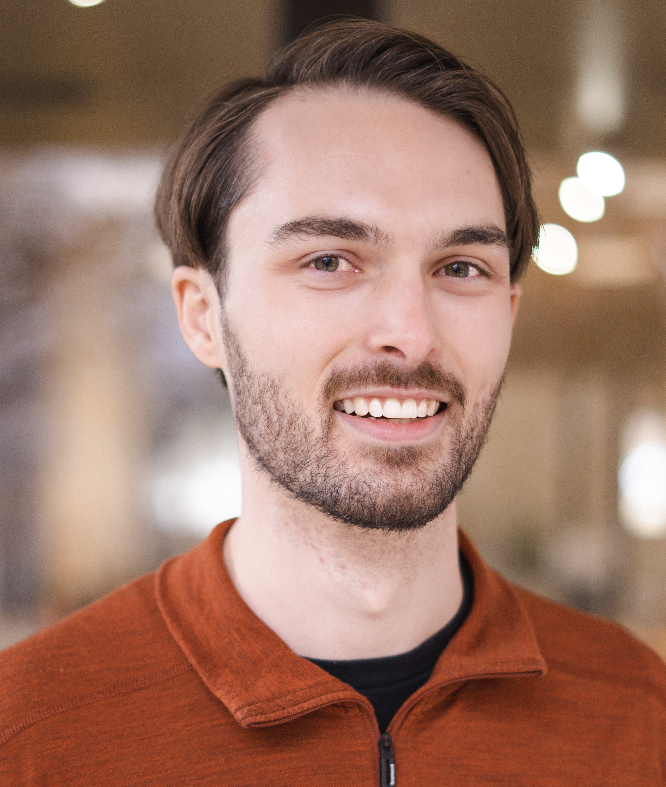
\includegraphics[width=0.7\textwidth]{headshot-small.png}
        \end{column}
    \end{columns}
\end{frame}

\begin{frame}{Why the Observatory on Social Media?}
    \vfill
    \begin{columns}
        \begin{column}{0.5\textwidth}
            Want to do more applied work \\
            \vspace{5mm}
            
            Past experience with social media:
            \begin{itemize}
                \item Large-scale analysis of Twitter data
                \item Collaborations with journalism scholars
                \item Two internships at Facebook
            \end{itemize}
            
            \vspace{4mm}
            Curious about social dynamics in science
        \end{column}
        \begin{column}{0.5\textwidth}
            \centering
            \includegraphics[width=0.87\textwidth, page=2]{citations.pdf}
        \end{column}
    \end{columns}
\end{frame}

\begin{frame}{My background is in statistical methods development for networks}
    \vfill
    \begin{columns}
        \begin{column}{0.5\textwidth}
            Projects so far:
            \begin{itemize}
                \item PCA + neural nets to embed networks
                \item Embeddings for causal inference
                \item Contagion and peer effects
                \item Causal machine learning (a little)
            \end{itemize}
        \end{column}
        \begin{column}{0.5\textwidth}
            \centering
            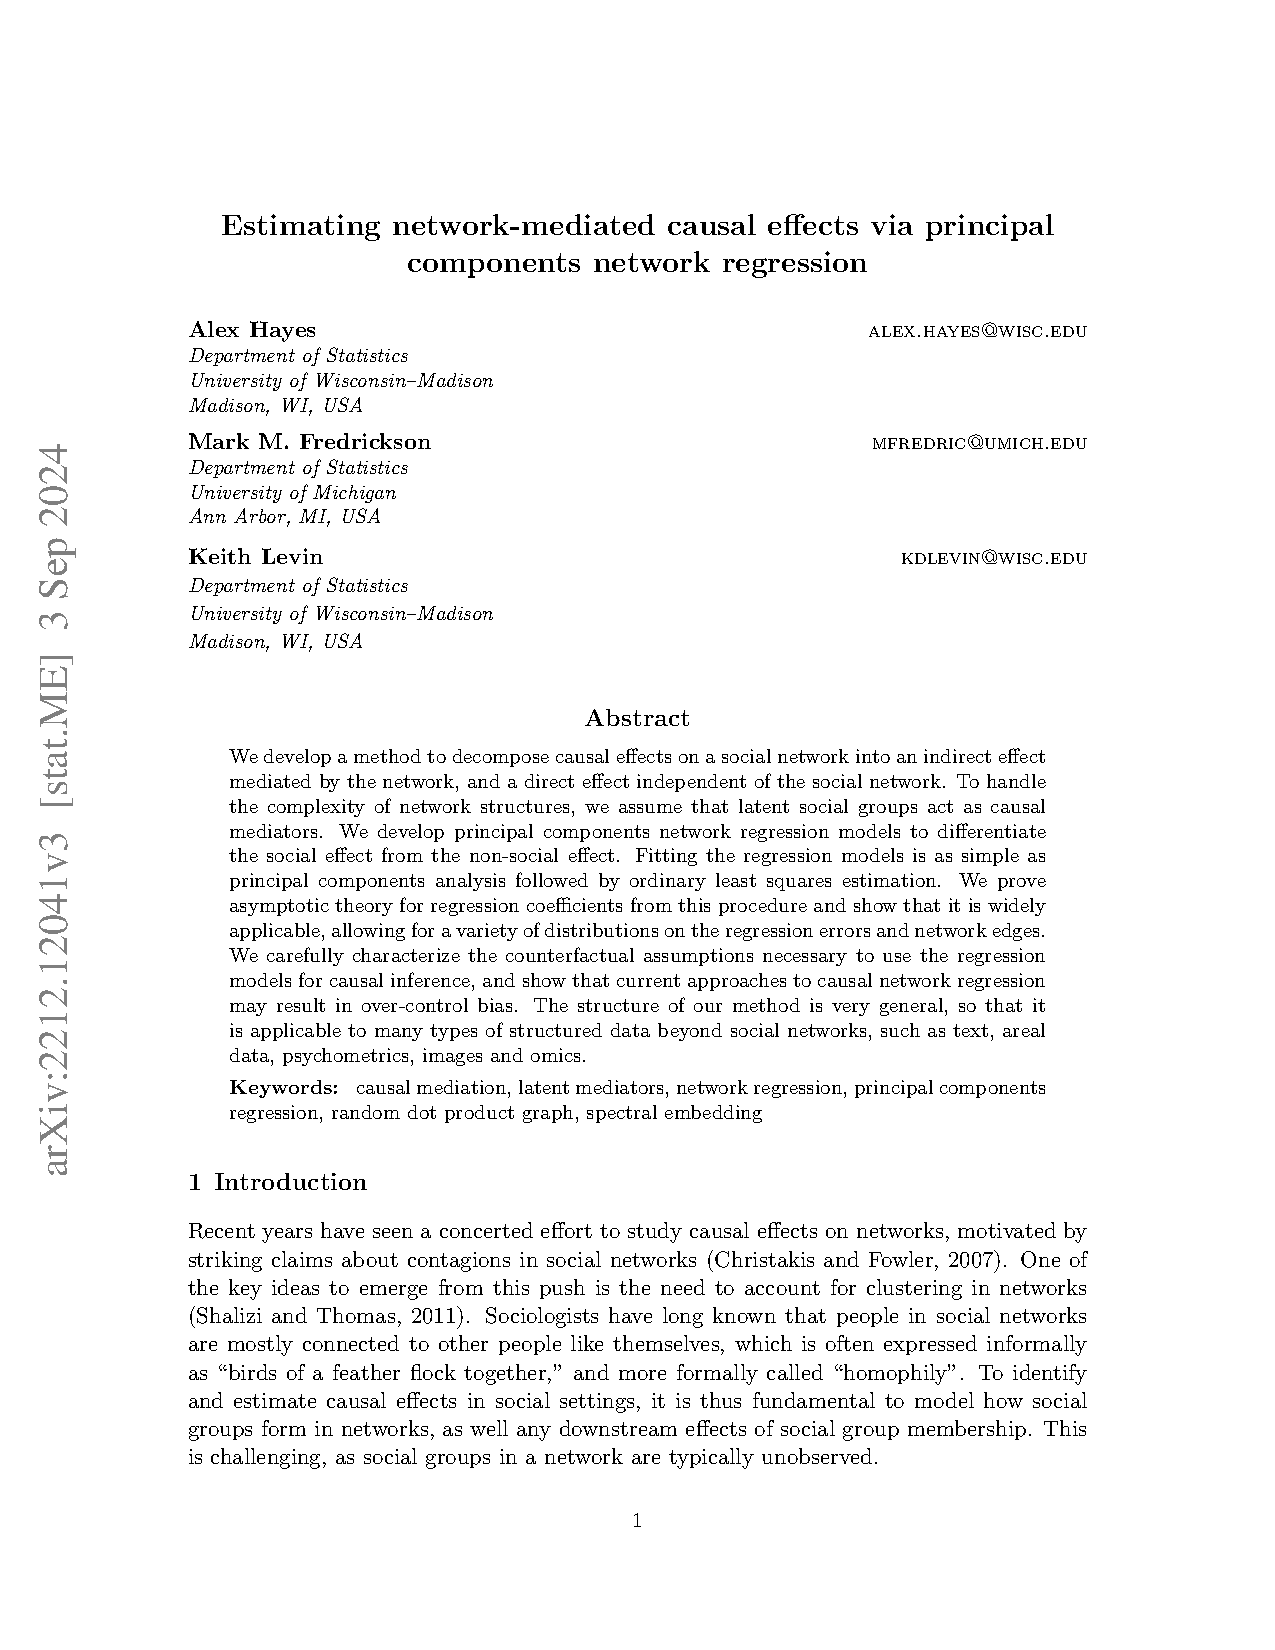
\includegraphics[width=0.92\textwidth, page=1]{mediation.pdf}
        \end{column}
    \end{columns}
\end{frame}

\begin{frame}{I write a lot of code}
    \vfill
    \begin{columns}
        \begin{column}{0.55\textwidth}
            \begin{itemize}
                \item Background in open-source development
                \item Nine \texttt{R} packages on CRAN
                \item Thousands of lines of \texttt{Python} running daily at Facebook
                \item Use Github and build system everyday
                \item Some C++ experience (speeding up slow linear algebra)
            \end{itemize}
        \end{column}
        \begin{column}{0.45\textwidth}
            \centering
            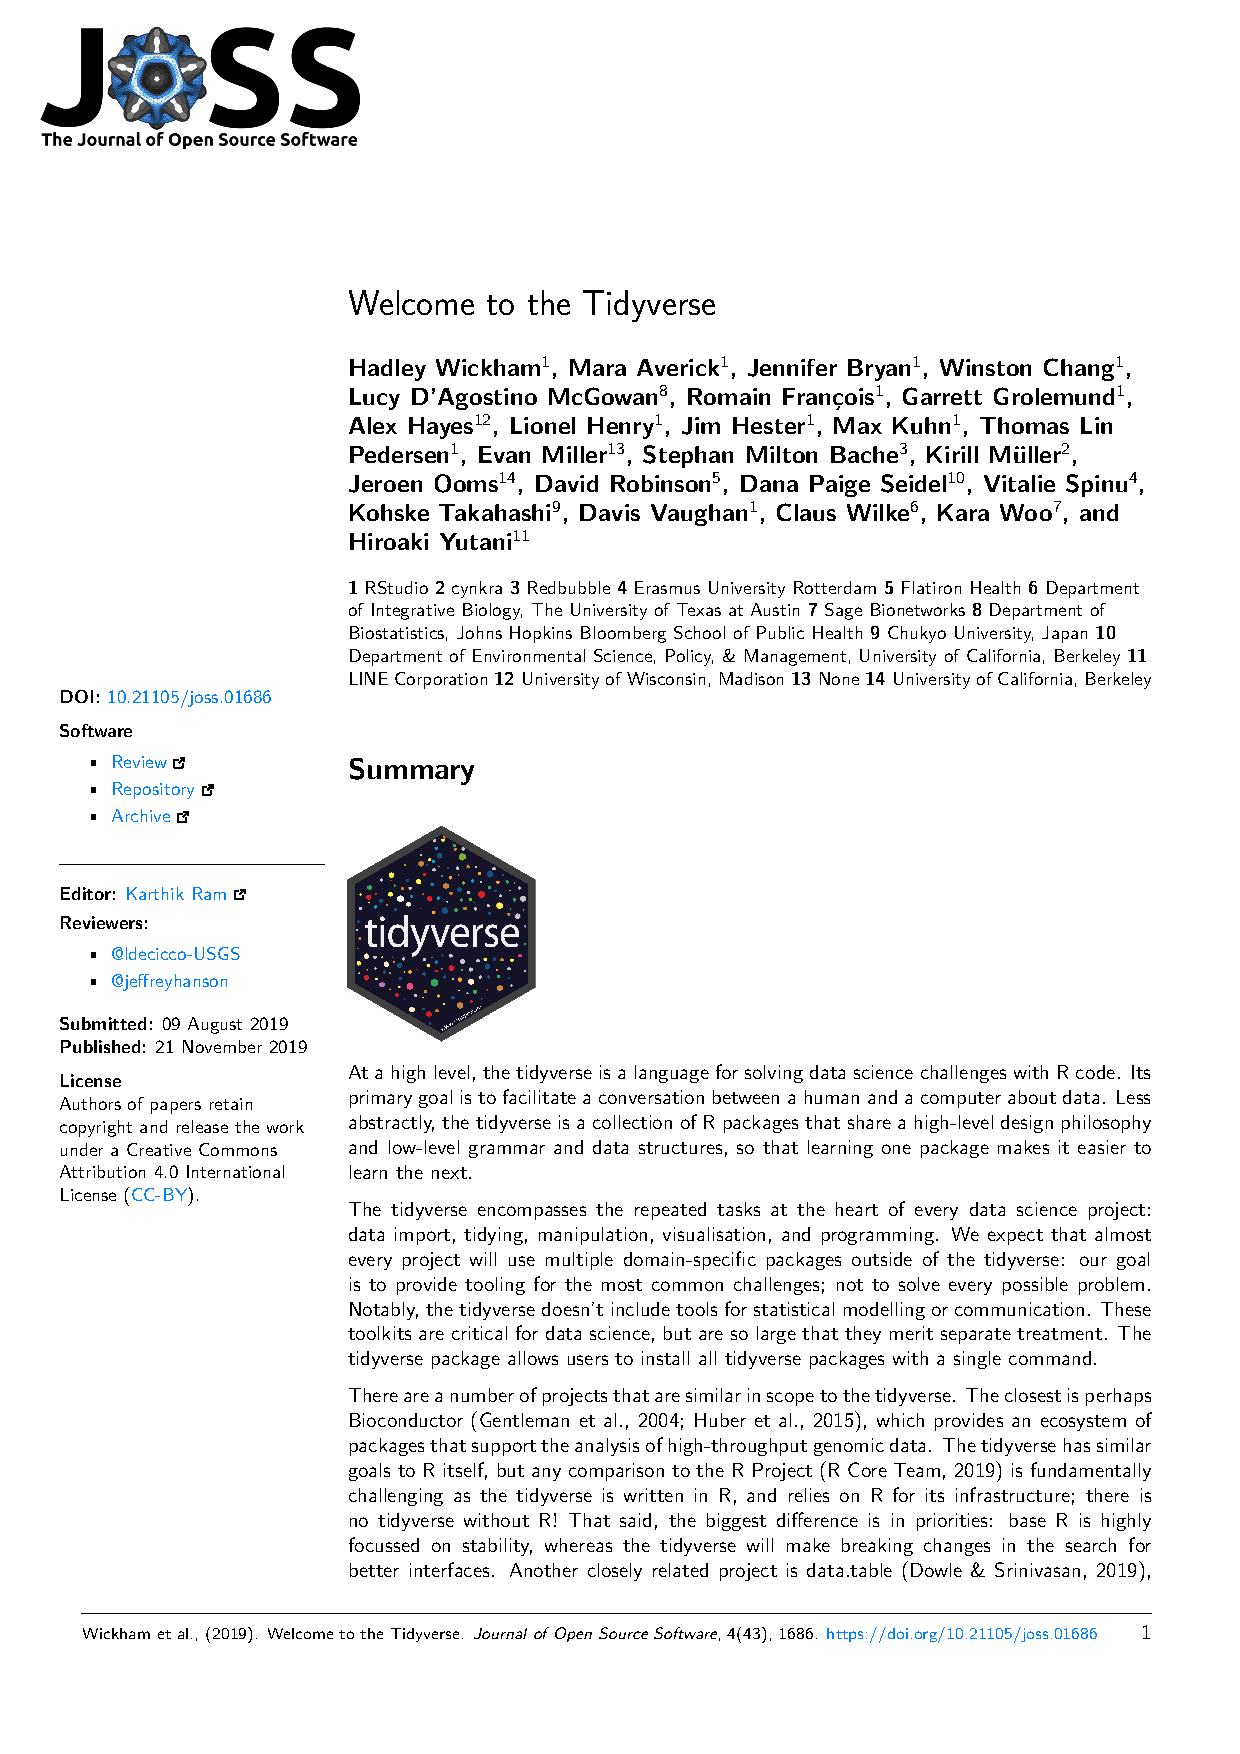
\includegraphics[width=0.8\textwidth, page=1]{tidyverse.pdf}
        \end{column}
    \end{columns}
\end{frame}

\begin{frame}{My vision for the future}
    Continue ongoing research:
    \begin{itemize}
        \item Estimating peer effects in noisy networks
        \item Estimating peer effects in dynamic networks
    \end{itemize}
    \vspace{4mm}
    
    Big picture goals:
    \begin{itemize}
        \item Develop new vein of research via postdoc
        \item Tenure-track faculty position
    \end{itemize}
\end{frame}

\nocite{hayes2024a,hayes2024b,hayes2024c,wickham2019}
% https://tex.stackexchange.com/questions/624177/biblatex-and-beamer-create-unwanted-references-in-header
\printbibliography[heading=none]


% Interview session; committee will ask some combination of the following:
% What are your career goals? Why OSoMe/IU? 
% Why are you interested in this NSF APTO project?
% What are you really good at professionally? What do you enjoy the most?
% What are you not good at or not interested in? What were the low points of your career?
% What were your biggest mistakes? What did you learn from them?
% What is an (or the most)  important question in your research area and why? Ideally, what would be needed to address it?
% Who were your senior colleagues in the past? How will they rate your research performance on a 1-10 scale when we talk to them? Why?
% Are you comfortable with software engineering and managing software projects? How do you manage your code and data? What do you do to ensure the reproducibility of your research?
% Do you have any experience in machine learning and embedding? 
% What are the most data- or computation-intensive computations you did?
% Have you had any opportunity to mentor junior students/collaborators? 
% During your postdoc appointment, would you be interested in teaching a course or writing grant proposals? Or would you prefer focusing on research?
% Do you prefer working alone or in a group? In the office or at home?

\end{document}